\documentclass[10pt,twocolumn,letterpaper]{article}

\usepackage{cvpr}
\usepackage{times}
\usepackage{epsfig}
\usepackage{graphicx}
\usepackage{float}
\usepackage{amsmath}
\usepackage{amssymb}

% Include other packages here, before hyperref.

% If you comment hyperref and then uncomment it, you should delete
% egpaper.aux before re-running latex.  (Or just hit 'q' on the first latex
% run, let it finish, and you should be clear).
\usepackage[breaklinks=true,bookmarks=false]{hyperref}

\cvprfinalcopy % *** Uncomment this line for the final submission

\def\cvprPaperID{****} % *** Enter the CVPR Paper ID here
\def\httilde{\mbox{\tt\raisebox{-.5ex}{\symbol{126}}}}

% Pages are numbered in submission mode, and unnumbered in camera-ready
%\ifcvprfinal\pagestyle{empty}\fi
\setcounter{page}{1}
\begin{document}

%%%%%%%%% TITLE
\title{Multi-factor Time-series Predication of Bitcoin Price}

\author{Yafeng GUO\\
Illinois Institute of Technology\\
10 W 35th St, Chicago, IL 60616\\
{\tt\small yguo82@hawk.iit.edu}
% For a paper whose authors are all at the same institution,
% omit the following lines up until the closing ``}''.
% Additional authors and addresses can be added with ``\and'',
% just like the second author.
% To save space, use either the email address or home page, not both
% \and
% Second Author\\
% Institution2\\
% First line of institution2 address\\
% {\tt\small secondauthor@i2.org}
}

\maketitle
%\thispagestyle{empty}

%%%%%%%%% ABSTRACT
\begin{abstract}
   Bitcoin is a cryptocurrency invented in 2008 by an unknown person or group of people using the name Satoshi Nakamoto ~\cite{Authors03}. 
   It is now the most popular form of cryptocurrency in the world, and is now being included in institutional investment 
   portfolios. How to predicate bitcoin price precisly is an interesting and valuable question. This article explored serveral 
   critical drivers behind bitcoin price and also validated diffrent predication approaches, like ARIMA and RNN.
\end{abstract}

%%%%%%%%% BODY TEXT
\section{Introduction}
Bitcoin is a cryptocurrency invented in 2008 by an unknown person or group of people using the name Satoshi Nakamoto. The currency began 
use in 2009 when its implementation was released as open-source software. Bitcoin is a decentralized digital currency, without a central 
bank or single administrator, that can be sent from user to user on the peer-to-peer bitcoin network without the need for intermediaries.
Transactions are verified by network nodes through cryptography and recorded in a public distributed ledger called a blockchain. Bitcoins 
are created as a reward for a process known as mining. ~\cite{Authors03} ~\cite{Authors04}. 

Bitcoin price has grown more than 5 times since beginning of 2020 (from 9367.4 USD to a new high 61,468.0 USD in Mar 2021). It 
attracted more and more attentions in the world. However, not all pepole have consensus on its value. The ex-president of US Donald Trump 
said digital currencies are "not money" and the value of bitcoin and cryptocurrencies are based on “thin air”. Whereas Elon Musk 
said he is "a Bitcoin Supporter" and accept "buy a Tesla with bitcoin". Those conflicted statements somehow can explain the price 
volatility of bitcoin, which bring challanges to bitcoin price predication.

Since outbreak of Covid-19 pandemic, the bitcoin price surged (Figure 1). A research conducted in ~\cite{Authors01} reflected 
that the portion of "investor-held Bitcoin" raised to 77$\%$ since 2017. The institutional investors treat bitcoin not so much 
as a currency, but as a hedge against macroeconomic uncertainty. According to analysis in ~\cite{Authors02}, 
the trend of considering bitcoin as a hedge in the long run emerged already in 2017. Bitcoin has become a new type of safe haven asset. From this 
of view, prices of other assets categories should have correlations with Bitcoin price. In this article, gold price, SP500 Index, Shanghai Stock 
Market Index, major currencies exchange rate are included as factors of macroeconomic.

\begin{figure*}[htb]
\begin{center}
\fbox{
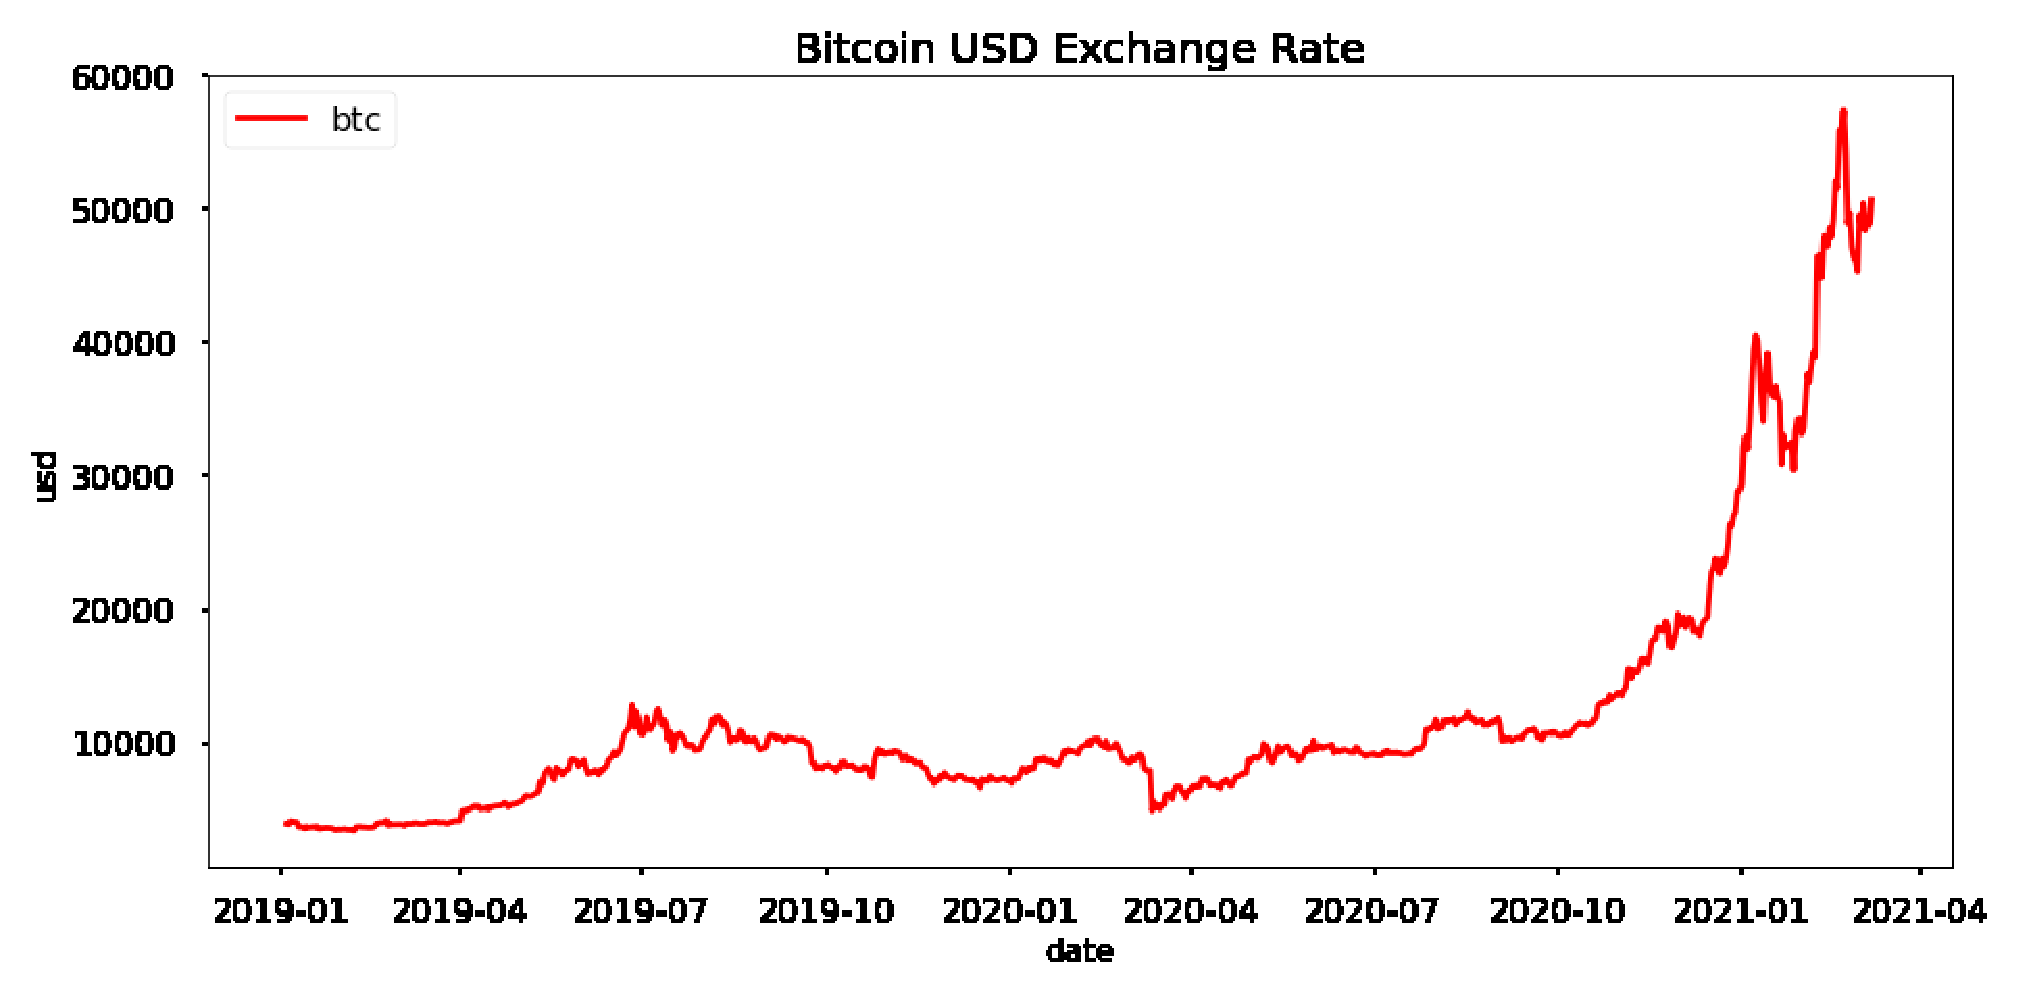
\includegraphics[width=0.8\linewidth]{figure1.eps} 
}

\end{center}
   \caption{Bitcoin USD exchang rate raised more than 6 times, since Jan 2019 to Mar 2021.}
\label{fig:long}
\label{fig:onecol}
\end{figure*}

Personal investors contributed major transactions in terms of transaction numbers. Personal investors shared the drivers behind institutional investors. Besides that, 
the public media impact has to be evluated as well. In this article, google trend are included to represent public media impact.  Baidu Index is also included as Google 
service is not avaiable in China.


%-------------------------------------------------------------------------
\subsection{Research Questions}

In short, the research question of this article is: { \bf With what accuracy level can the next day price 
of Bitcoin be predicted using which machine learning method? }



\subsection{Evaluation Method}

The question can be defined as a regression question, e.g. what is the exact price of next day ( I will use close price of every day in China Standard Time) . 
In this case the root mean squared error (RMSE) can be used as measurement. Besides the exact price, investors may also have intersting to know if the predicated trend is correct, 
e.g. it will go up, go down, or be flat tomorrow. The revert of growing trend or the reverting of decreasing trend are even more cirtical. We will use both RMSE and trend predication 
accuracy (TPA in short) to evaluate our models.

The formula of RMSE is defined as below: 

\par
\begin{equation*}
RMSE = \sqrt{\frac{\sum_{i=1}^{n}(Y_i - \hat{Y_i})^2  }{n}}
\end{equation*}

Here $ n $ is the number of samples, and $ Y_i $ is the true value in test set, and $\hat{Y_i}$ is the predicated value.

\par

The formula of TPA is defined as below:

\begin{equation*}
TPA = \frac{correct\ predication\ of\ peaks\ or\ troughs}{number\ of\ peaks\ +\ number\ of\ troughs } 
\end{equation*}




%------------------------------------------------------------------------
\section{Releated Work}

Although bitcoin has more than 10 years history, many pepole only become familiar with that since 2018 after bicoin exceeded 10,000 USD. 
And most articles I found on bitcoin price predication were around 2018. As machine learning got very fast development in those years, 
leveraging latest machine learning technology to do such research will be interesting.

In ~\cite{Authors05}, Obryan Poyser explored determinants of bitcoin price. Obryan seperated bitcoin price drivers to internal drivers and external drivers.
For internal dirvers, it is mainly about transaction volume, hash rate etc. Obryan actally spend a considerable research effort on external factors. 
Obryan found bitcoin price has correlation with gold price, stock maket, currency exchange rate, investors' sentiment etc. He used traditional 
shallow machine learning algorithms, and get an error level at 3.146$\%$.

As bitcoin prices changed very frequently and sharply in 2021, it will be hard to achieve the error level in case we want to predict bitcoin prices
for 2021. However, the bitcoin prices drivers won't change dramtically. So our predicating factors are mostly inspired by Obryan's work.


H. Jang et al. used rolling window LSTM model to predicate bitcoin prices in 2018 ~\cite{Authors06}. They mainly include blockchain information and macroeconomics information like exchange rate to do the predication. They compared different machine learning algorithm like SVR, LR etc. They don't have a comparison with typical time-series algorithm like ARIMA, VAR etc. From their experiment, rolling window LSTM is a promising model for bitcoin price predication.

H. Jang et al. used a modern NN approach to do the predication, however they don't include  traditional time-series algorithm as a benchmark. Another thing we want to mention is they didn't consider emotional drivers. Speculative investors are sensitive to public emotion. Including search index, social media emotional analysis could be helpful for accurate predication.




%------------------------------------------------------------------------
\section{Predication Models}
Here we will introduce our work on bitcoin predication. In the first section, we will introduce the data sources we will use and also data pre-processing we adopted. We build two models to do the predication. One is ARIMA model, which used only history of bitcoin prices to do the predication. ARIMA is a popular model to do the time-series predication. We will use it as a benchmark. Another model we will build is LSTM. We will include multiple factors to do the predication with LSTM. We will prove LSTM is a better method to do the predication.



\subsection{Dataset and Data Processing}
 
We used following dataset to do the predication:
%-------------------------------------------------------------------------
\begin{itemize}
\item[$\bullet$] Bitcoin price data - www.investing.com
\item[$\bullet$] Gold price data - www.investing.com
\item[$\bullet$] SP500 data - www.investing.com
\item[$\bullet$] Shanghai Strock data - www.investing.com
\item[$\bullet$] USD to CNH exchange rate data - www.investing.com
\item[$\bullet$] EUR to USD exchange rate data - www.investing.com
\item[$\bullet$] EUR to CNH exchange rate data - www.investing.com
\item[$\bullet$] Baidu index data with keywords "Bitcoin" (in Chinese) - index.baidu.com
\item[$\bullet$] Google search trend with keywords “Bitcoin” - trends.google.com
\end{itemize}

As we are familiar with SQL language, we decided to import all data we got into a SQLite database[add refer to SQLite]. Our models will retrieve data from SQLite database and we could filter out date range we are interesting in with SQL language. A free database manage tool Dbeaver[add refer to DBeaver] is leveraged to explore and manage data in the SQLite database.

As we used stock market index as our modelling features, and stock market is closed at the weekend. We will simply fill the weekend stock market index using the close index of last Friday.

Google trends will provide only monthly data if the time range crossed more than two years. A tool ~\cite{tool01} were used to retrive daily data.

\subsection{ARIMA}

In this section we will implement a seasonal ARIMA model to predicate bitcoin price. We will first give a brief introduction on seasonal ARIMA. Later we will cover details of seasonal ARIMA modelling, and then give a short summary.
{}
\subsubsection{ARIMA Introduction}

The ARIMA model was introduced by George Box and Gwilym Jenkins in their textbook Time Series Analysis: Forecasting and Control in 1970. It also referred to as Box-Jenkins methodology, and is a very popular method to do time-series predication, especially for finicial forecasting. You can refer to an online book ~\cite{Authors07} by Rob and George for more details.

ARIMA stands for AutoRegressive Integrated Moving Average. It is a generalization of the simpler AutoRegressive model and Moving Average model with integration.

\paragraph{AutoRegressive model}
\par
AutoRegressive model leveraged historical observations to predict future value. It assume the data it is observing are stationary, e.g the mean and variance of data has no dependency on time. In this case, it can forecast the future value using following formula:
\par
\begin{equation*}
y_t = \mu + \sum_{i=1}^{p}\gamma_iy_{t-i} + \epsilon_t{}
\end{equation*}
Here $y_t$ is the forecast value, $\mu$ is a constant value, $p$ is called AR order, meaning how many preceeding observances have impact on current value. $\gamma_i$ is  coefficients and $\epsilon_t$ is residual error.

\paragraph{Moving Average}
\par
If we look at AutoRegressive model, we will find the residual error is something we can not ignore. If in time step $t - 1$ there is a white noise, which will impact time step $t$, and it will propagate to time step $t + 1$, the white noise will have very significant impact on predications. Moving average model is used to handle residul errors. It assume the future value we want to predicate is impacted by previous residual errors. 

\par
\begin{equation*}
y_t = \mu + \epsilon_t + \sum_{i=1}^{q}\theta_i\epsilon_{t-i} 
\end{equation*}

Here $y_t$ is the forecast value, $\mu$ is a constant value, $q$ is called MA order, meaning how many preceeding residual errors have impact on current value. $\theta_i$ is coefficients and $\epsilon_t$ is residual error.

Moving average model is taking residual error into predication consideration, which will improve predication accuracy.

\paragraph{Integration}
\par
AutoRegressive model assume data are stationary, but which is not the case in most time. We need some tricks to make data stationary. Integration assume if we subtract previous observations from value of current time step, the data will become stationary. We usually use d to notate the order of integration (e.g. the number of times doing differencing).

\paragraph{ARIMA}
\par
ARIMA is a combination of above three. ARIMA model can be (almost) completely summarized by three numbers: 
\begin{equation*}
	\begin{aligned}
	&p\ =\ \#\ of\ autoregressive\ terms \\ 
	&d\ =\ \#\ of\ nonseasonal\ differences \\  
	&q\ =\ \#\ of\ moving-average\ terms 
	\end{aligned}
\end{equation*}

\par

This is called an “ARIMA(p,d,q)” model. 

For example, ARIMA(1,1,2) means

\par
\begin{equation*}
y_t = \mu + \epsilon_t + \gamma y_{t-i} + \phi(y_{t-1} - y_{t-2} ) + \sum_{i=1}^{2}\theta_i\epsilon_{t-i} 
\end{equation*}



\paragraph{Seasonal ARIMA}
\par
Seasonal is an ARIMA model which further include seasonal factors into consideration. For example, personal bank account balance may have monthly changes because he or she receive salaries periodically. When we do account balance predicating, include seasonal factors into consideration will be very helpful.
We can use exactly same parameters to describe seasonal components of the time-series data. e.g. We can add three additional numbers: 

\begin{equation*}
	\begin{aligned}
	&P\ =\ \#\ of\ seasonal\ autoregressive\ terms \\ 
	&D\ =\ \#\ of\ seasonal\ differences \\  
	&Q\ =\ \#\ of\ seasonal\ moving-average\ terms 
	\end{aligned}
\end{equation*}

\par

The complete model is called an “ARIMA(p,d,q) $\times$ (P,D,Q)” model.

\subsubsection{Seasonal ARIMA model implementation}
\par
As we said above, to build a seasonal ARIMA model, we have 6 critical hyper parameters to identify. In the first step below, we will verify the seasonal component of bitcoin price (from Jan 2019 to Mar 2021). Through seasonal components analysis, we will identify 3 parameters related to seasonal components. After that, we will do necessary transformation and differences to make the time-series data stationary. During this step, we will find a right value for parameter $d$. After that, we will search through the hyper parameters spaces to right find $p$ and $q$, and find a best model with right coeffcients for each term.

\paragraph{Seasonal components analysis}
We used $statsmodels.api.tsa.stattools.adfuller$ to do a Dickey-Fuller stationary test. The test result is $1.000$, which indicate the data is not stationary at all. We also used $statsmodels.api.tsa.seasonal\_decompose$ to do the seasonal components analysis. Figure 2 illustrated the analysis result. From the chart we can find bitcoin prices contains very few seasonal components, it is even less significant than residual errors. Hence we could ignore seasonal components. In this case, we can simply to $(P, D, Q)$ to $(0, 0, 0)$

\begin{figure*}[h]
\begin{center}
\fbox{
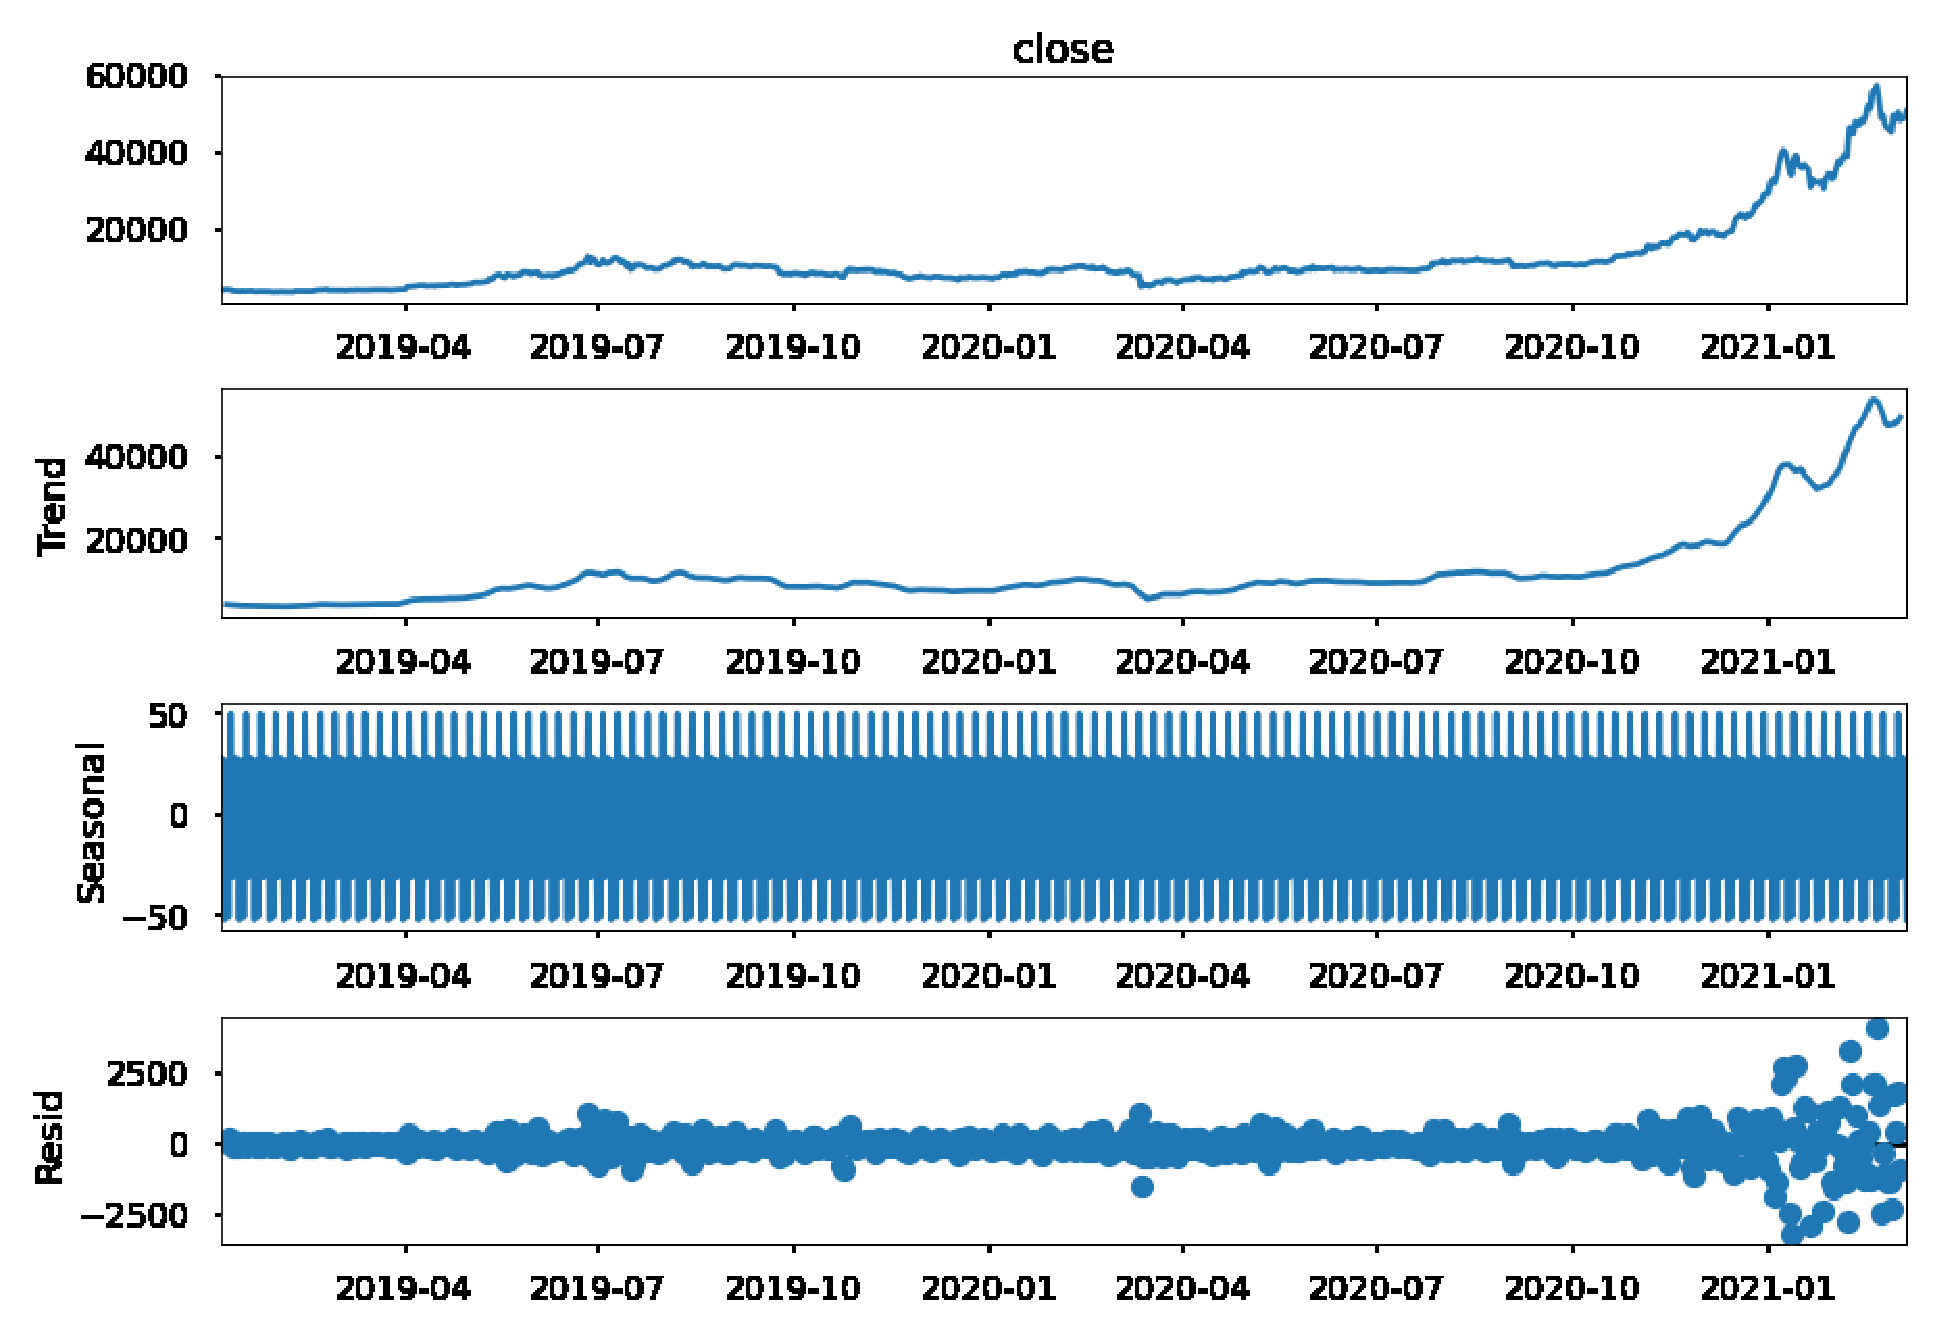
\includegraphics[width=0.8\linewidth]{figure2.eps} 
}
\end{center}
   \caption{Seasonal components analysis of bitcoin price. Seasonal components are not significant.}
\end{figure*}

\paragraph{Stationary check and transformation}
As the time-series data is not stationary by default, and the growth of bitcoin price is near to an exponential growth, we do a $boxcox$ transformation. After that do a one order difference to make data stationary. Figure 3 show the result after transformation. We did another round Dickey-Fuller stationary test and its result is $0.000$, which means the data is stationary.

\begin{figure*}[h]
\begin{center}
\fbox{
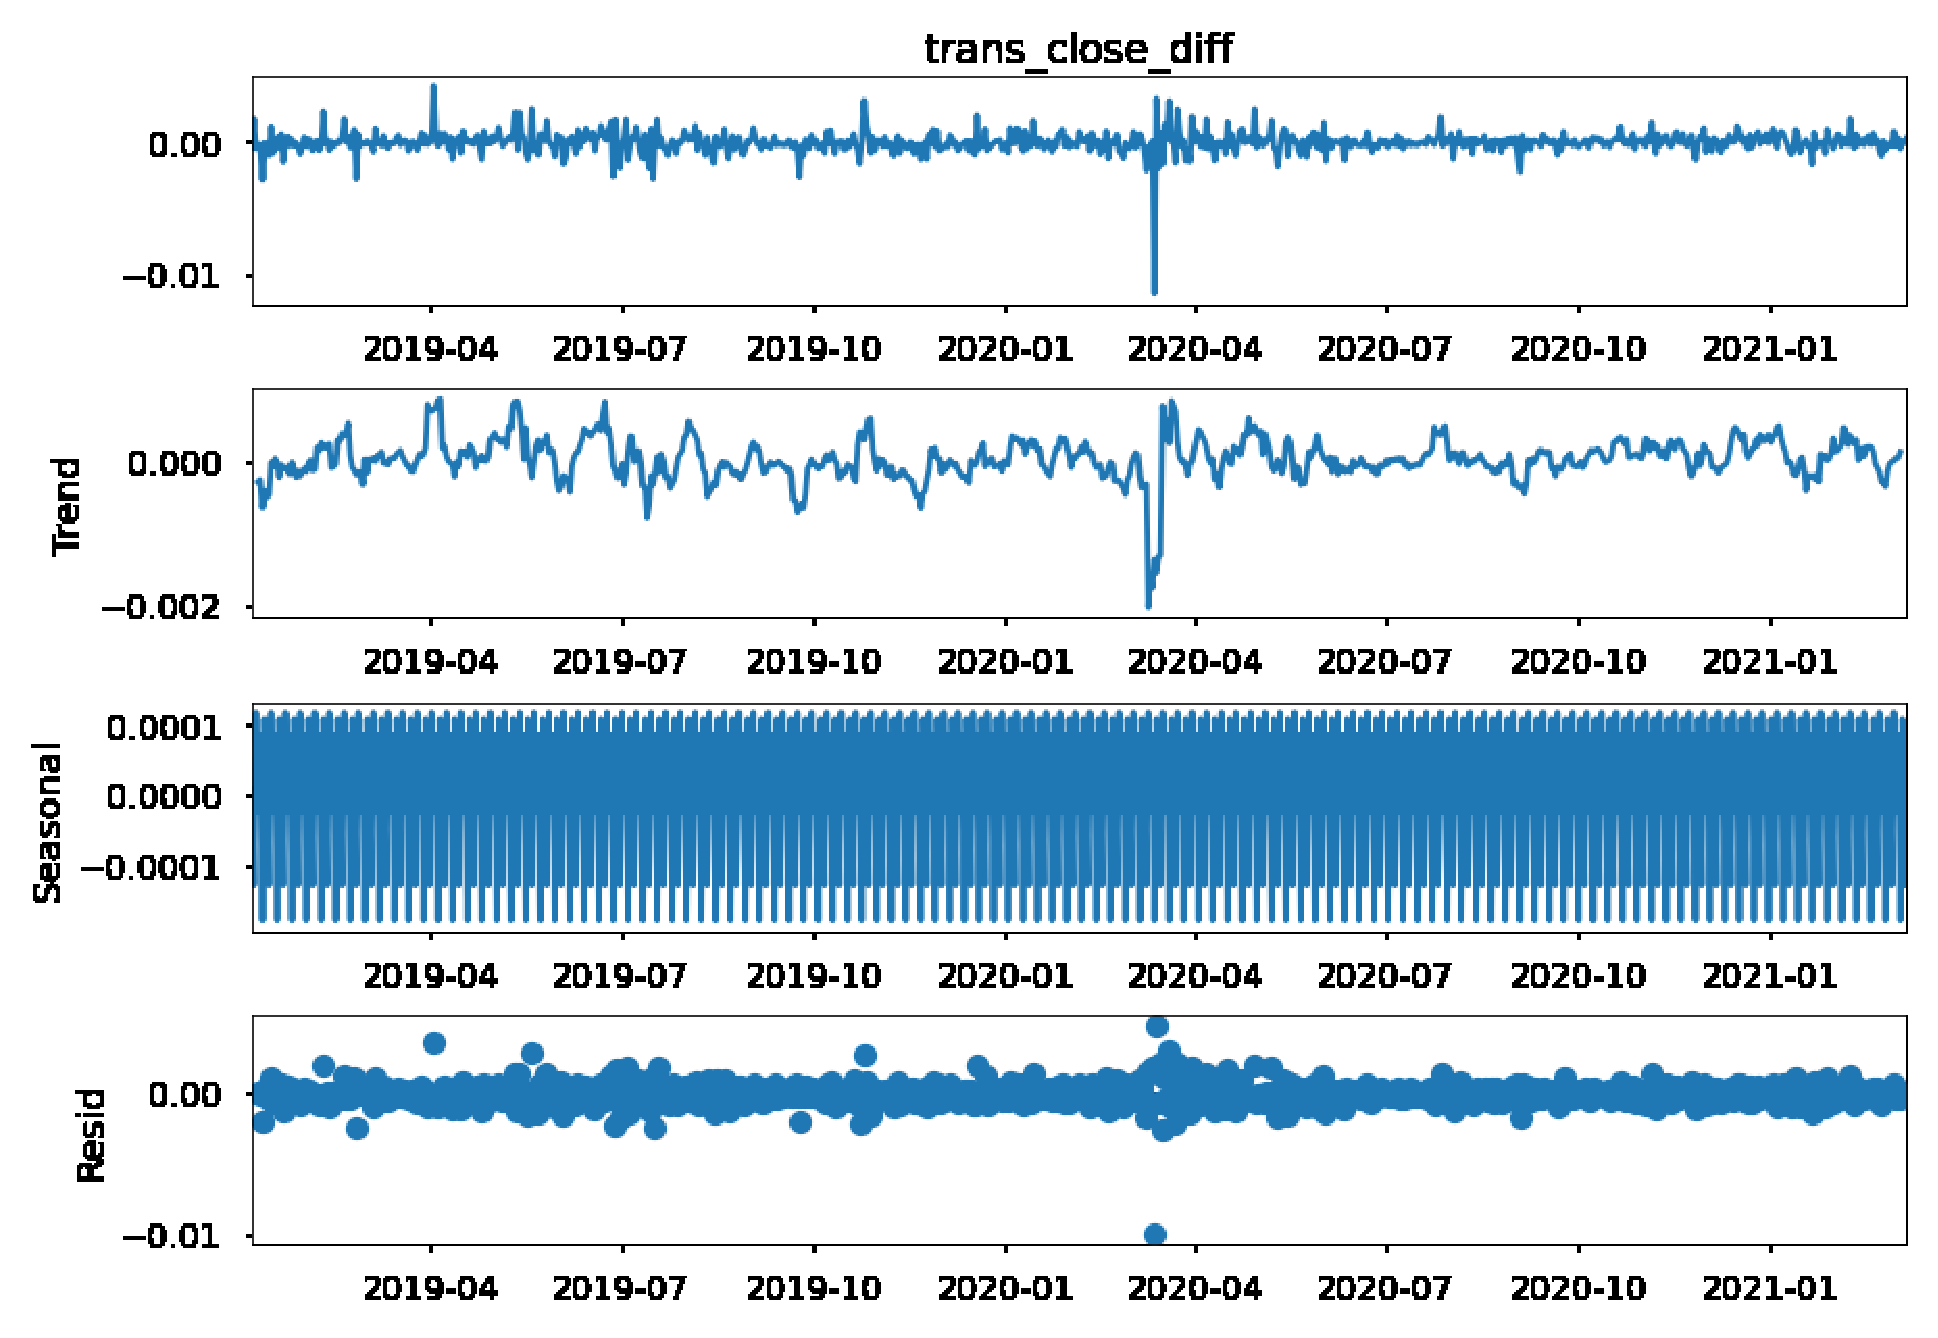
\includegraphics[width=0.8\linewidth]{figure3.eps} 
}
\end{center}
   \caption{Bitcoin price after boxcox transformation and one order difference. It becomes stationary after transformation.}
\end{figure*}

\paragraph{Searching best model}
Based on previous analysis, after a boxcox transformation, the parameter $d$ will be $1$. And parameters $(P, D, Q)$ will be $(0, 0, 0)$. Hence when searching models, we only need consider $(p, q)$. Supposing those two parameters can take values 0, 1, 2 respectively, we will have 9 combinations to search. Figure 4 illustrate the whole searching process. We will use AIC (Akaike Information Criterion) as the criteria to select models.

\begin{figure}[H]
\begin{center}
\fbox{
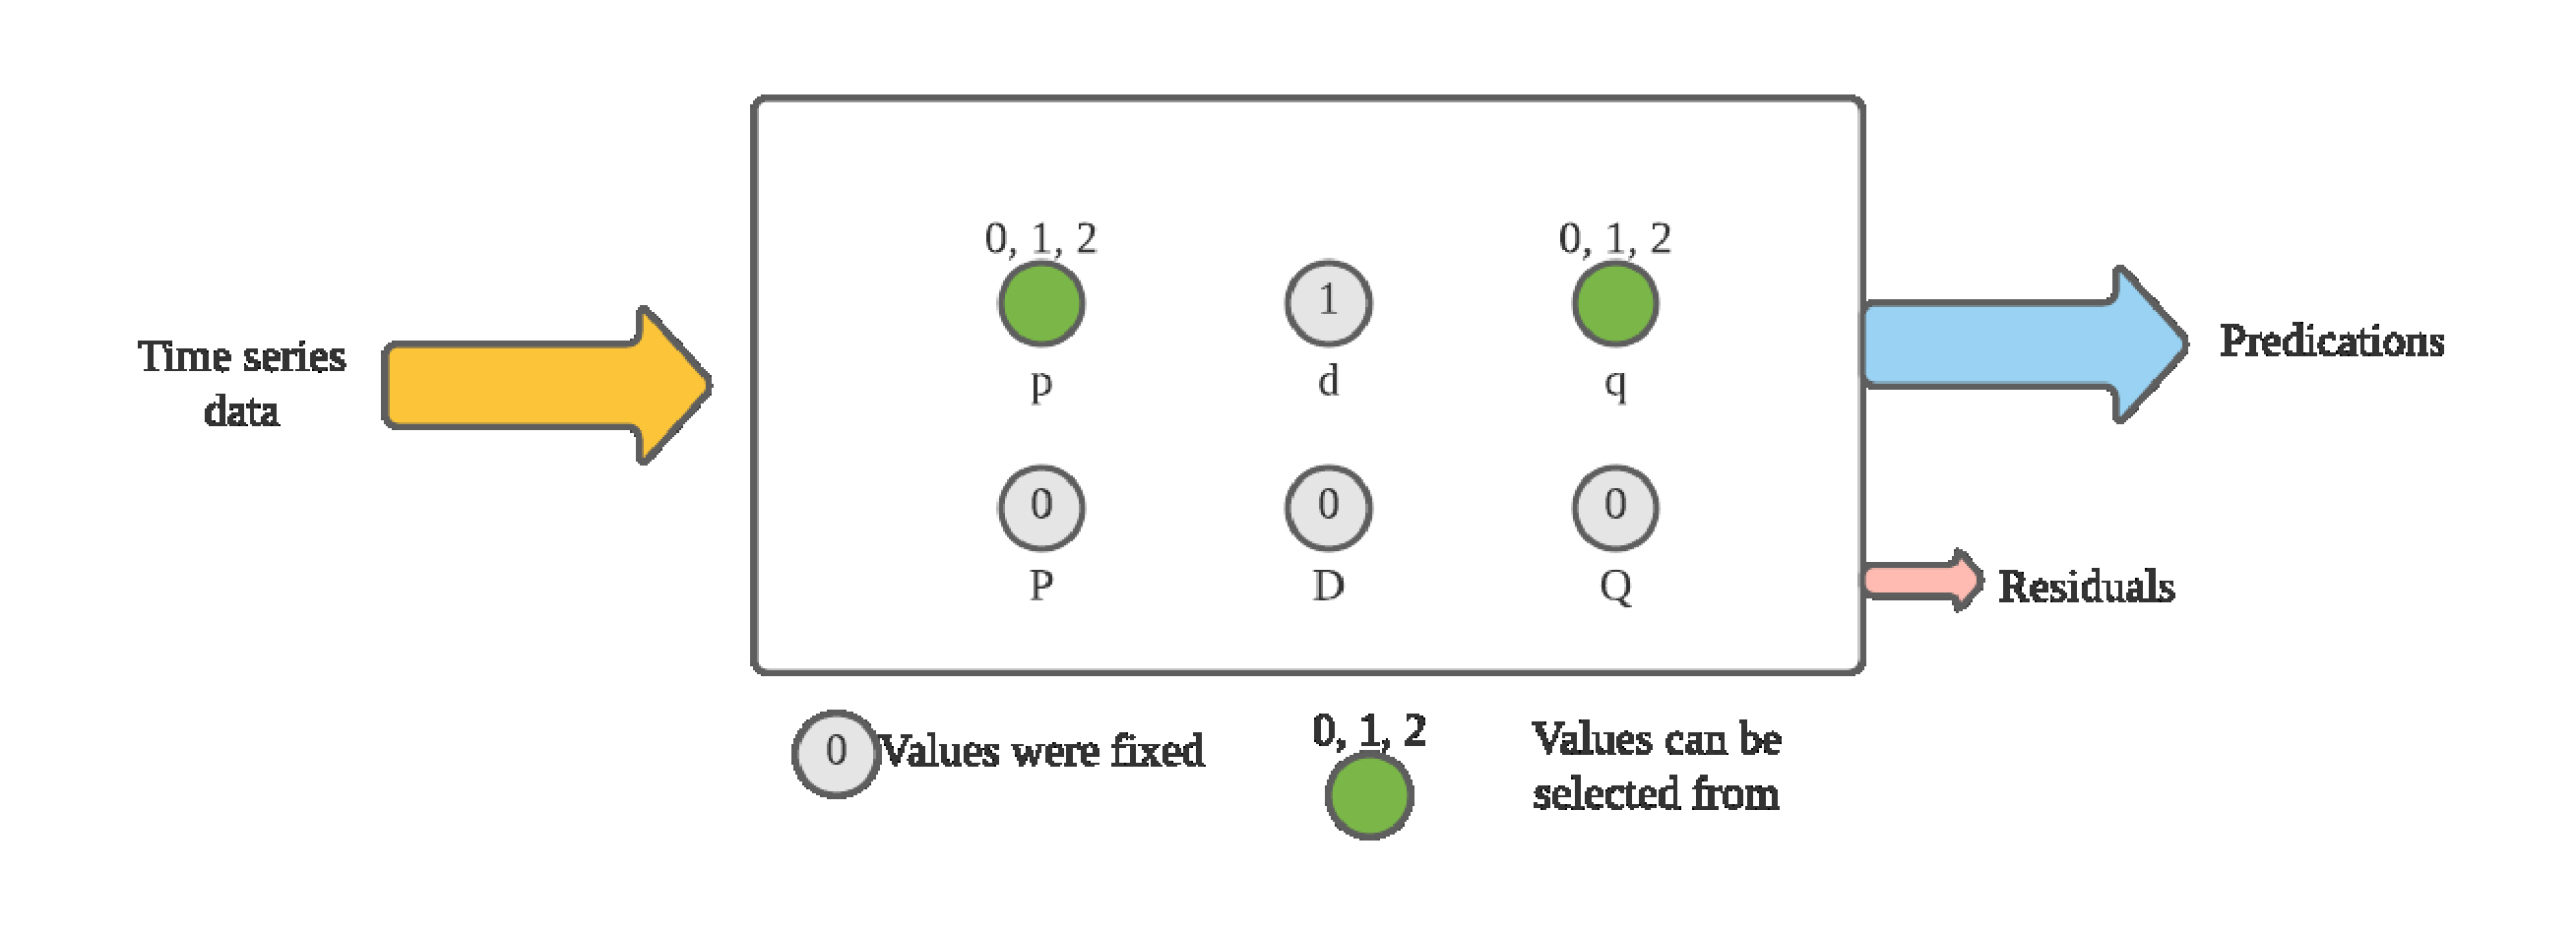
\includegraphics[width=0.8\linewidth]{figure4.eps} 
}
\end{center}
   \caption{Models Search~\cite{Authors08}. We will use AIC as criteria to choose models.}
\end{figure}


When we have a model fitted, we will use that predicate the value of next day only to improve predication accuracy. This is a kind of rolling window predication. When we finish a predication for a date, we will add the real data to train dataset and train a new model. We start the predication from Jan 12 2021, and predicated 43 days in total, which means we will train 43 models independently to do the predication. Figure 5 is the predication result.

\begin{figure}[H]
\begin{center}
\fbox{
\includegraphics[width=0.8\linewidth]{figure5.eps} 
}
\end{center}
   \caption{Predication result, from Jan 12 2021 to Feb 25 2021.}
\end{figure}

\paragraph{Summary}

The average RMSE of predication $50.21$. Which is $0.1\%$ of price value, it is very good. However, when we look at the TPA (Trend Predication Accuracy), it is $3.57\%$ only (1 of 28). The predication by ARIMA is almost just shift the real time-series data right by one time step, which makes it almost not useful for any investors.

We will continously explore LSTM modelling technology.

\subsection{Long short-term memory, LSTM}

In this section we will implement a LSTM model to predicate bitcoin price. We will first give a brief introduction on RNNs and LSTM networks. Later we will cover details of LSTM modelling, and then give a short summary.

\subsubsection{Recurrent Neuarl Networks}

Recurrent Neuarl Networks  or RNNs in short, are a type of neural network used to process and predicate sequential data. Time series data is a type of sequential data, hence RNNs are good network sturctures to handle them.

\paragraph{Vanilla RNNs Review}
\par
Recurrent neural networks were based on David Rumelhart's work in 1986~\cite{Authors10}. Both fully-connected network and CNN didn't capture the sequence information in the dataset. To precess sequential data, a straightforward thinking is we need feed previous time step output into current time step input. And that is Vania RNNs basic strubute. Please refer to figure 6. The left side of figure 6 is the most simple RNN. Input X got a transformation (with weight U) then we have the hidden state s, from one perspective, s got a transformation (with weight V) and generate output o of current timestep, and from another perspective, s was feed into next time step after a transformation (with weight W). the rigth side of figure 6 is the same RNN network which unfolded to all time steps.

\begin{figure}[H]
\begin{center}
\fbox{
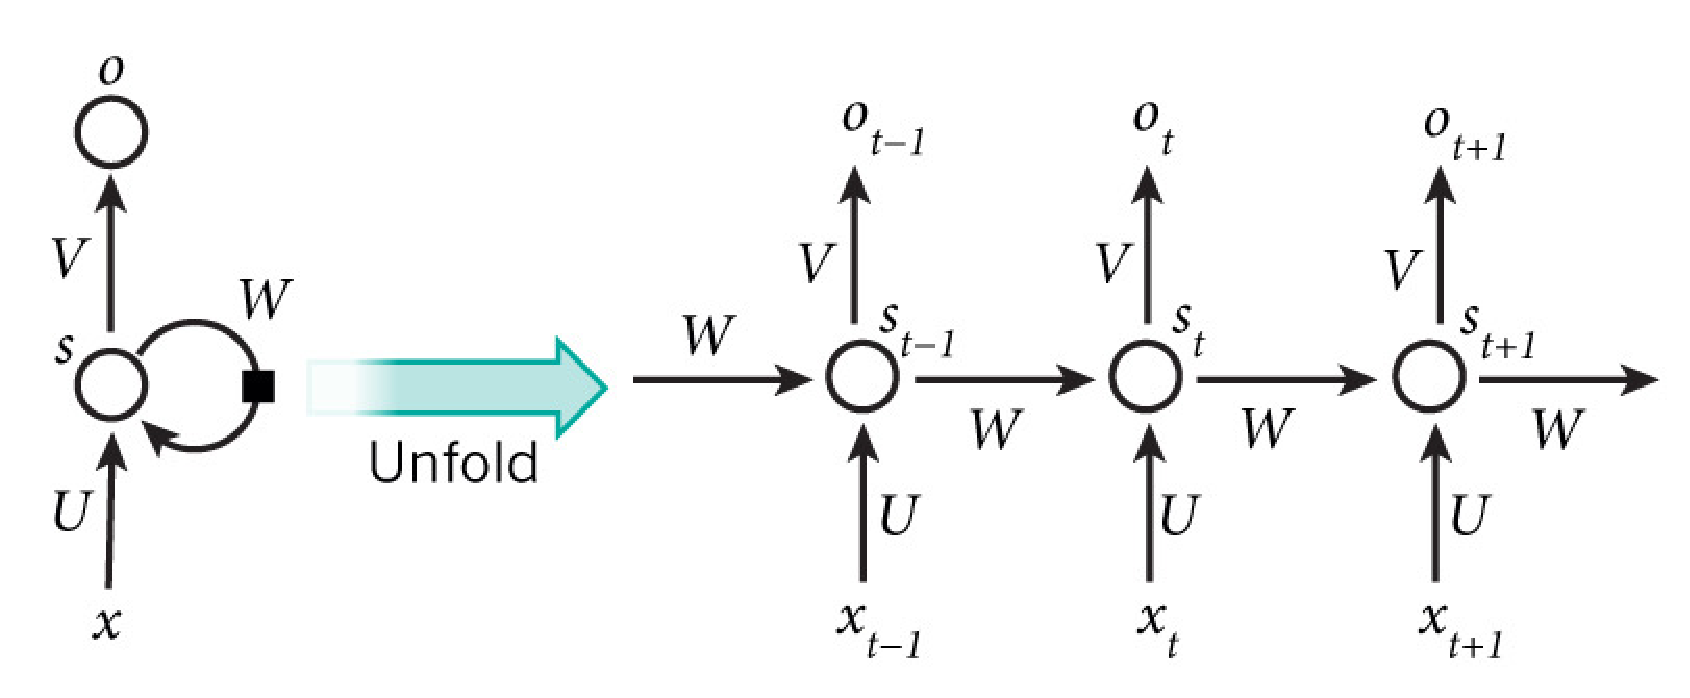
\includegraphics[width=0.8\linewidth]{basic_rnn.eps} 
}
\end{center}
   \caption{Vanilla RNecurrent Neural Netowrks\cite{Authors12}}
\end{figure}

\par
Vanilla RNNs are not able to handle long range dependency and also hard to train because the vanishing gradient and the exploding gradient problem. In practice, few pepole are using vanilla RNNs now.

\paragraph{LSTM Review}
\par

Long short-term memory (LSTM) networks were invented by Hochreiter and Schmidhuber in 1997\cite{Authors11}. Unlike vanilla RNNs cell can only pass one hidden state to next time step, LSTM cell can pass a hidden state and also a cell state. How can LSTM track long term dependency?

\begin{figure}[H]
\begin{center}
\fbox{
\includegraphics[width=0.8\linewidth]{lstm_main.eps} 
}
\end{center}
   \caption{Long short-term memory (LSTM) networks \cite{Authors12}}
\end{figure}


Please refer to figure 8. In one LSTM cell, there are three major components, called three "gates".

\begin{itemize}
\item[$\bullet$] The yellow $\sigma$ function accept current time step input $X_t$ and previous time step hidden state $h_{t-1}$. Its output will do a element-wise product with previous time step cell state $C_{t-1}$. This is called \textbf{"forget gate"}. The forget gate will control whether or not the previous cell state $C_{t-1}$ should be considered in current time step. If the output of forget gate is zero, that means the current time step will forget previous cell state.
\item[$\bullet$] The orange $tanh$ function will take current time step input $X_t$ and previous time step hidden state $h_{t-1}$ and generate an output $\tilde{C}_t$. The output $\tilde{C}_t$ is only an candidate. Whether or not it can be added into cell state, is controlled by the output of green $\sigma$ function. If the output of green $\sigma$ function is one, then $\tilde{C}_t$ will be added into cell state, combined together with portion of $C_{t-1}$ which passed forget gate. After the combination, we will get the cell state $C_t$ for this time step, The green $\sigma$ is called \textbf{"input gate"}.
\item[$\bullet$] The cell state $C_t$ will be passed to next time step, which will be controlled by forget gate of next time step. The red $\sigma$ function accept current time step input $X_t$ and previous time step hidden state $h_{t-1}$. Its output will do a element-wise product with result of $tanh$ function, which take current step cell state as input. The result of this element-wise product will become hidden state $h_t$ of current time step, and will be feed into next time step. The red $\sigma$ is called \textbf{"output gate"} as it control whether or not output cell state as hidden state.

\end{itemize}

All the parameters of those gate functions, activation functions will be trained through backpropagation. It is proven that it can overcome most challenges vanilla RNNs have. The drawback is it can be computationally expensive. Although we will not cover here, but GRUs discovered by Cho, et al. in 2014 relieved some computation cost issues.


\begin{figure}[H]
\begin{center}
\fbox{
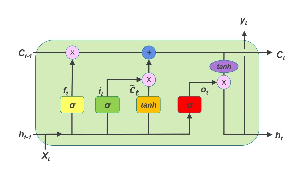
\includegraphics[width=0.8\linewidth]{lstm_cell.eps} 
}
\end{center}
   \caption{Long short-term memory (LSTM) networks cell structure \cite{Authors12}}
\end{figure}

\subsubsection{LSTM model implementation}
\par

\section{Conclusion}


\section{Future work}

In the future we will improve the preidciation from those two perspectives:

\begin{itemize}
\item[$\bullet$] Introduce more data dimensions. For example, introduce sentiment analysis on public media like Twitter, Weibo and open forums. We will try if adding more dimensions will improve prdication accuracy.
\item[$\bullet$] Try the predication with the latest time-series predication algorithms, like DeepAR etc.

\end{itemize}

The financial assets valuation predication is remaining a challanging problem and worth continous research on that.

\section{Appendeix}

The source code and dataset used in this paper can be found here: 
\par
https://github.com/yafengguo/cs584\_term\_paper.

{\small
\bibliographystyle{ieee_fullname}
\bibliography{egbib}
}

\end{document}
